
% JuliaCon proceedings template
\documentclass{juliacon}
\setcounter{page}{1}
\newcommand{\refalg}[1]{Algorithm~\ref{#1}}
\newcommand{\refsec}[1]{Section~\ref{#1}}
\newcommand{\reffig}[1]{Figure~\ref{#1}}
\newcommand{\refsubfig}[1]{Figure~\subref{#1}}
\newcommand{\reftab}[1]{Table~\ref{#1}}
\newcommand{\refeqn}[1]{(\ref{#1})}
\newcommand{\reflst}[1]{Listing~(\ref{#1})}

\begin{document}

% **************GENERATED FILE, DO NOT EDIT**************

\title{My JuliaCon proceeding}

\author[1]{1st author}
\author[1, 2]{2nd author}
\author[2]{3rd author}
\affil[1]{University}
\affil[2]{National Lab}

\keywords{Julia, Optimization, Game theory, Compiler}

\hypersetup{
pdftitle = {My JuliaCon proceeding},
pdfsubject = {JuliaCon 2019 Proceedings},
pdfauthor = {1st author, 2nd author, 3rd author},
pdfkeywords = {Julia, Optimization, Game theory, Compiler},
}



\maketitle

\begin{abstract}

Solving optimal power flow is an important tool in the secure and cost
effective operation of the transmission power grids. \lstinline{ExaPF.jl} aims to
implement a reduced space method for solving the optimal power flow problem (OPF)
fully on GPUs. Reduced space methods enforce the constraints, represented here by
the power flow's (PF) system of nonlinear equations, separately at each
iteration of the optimization in the reduced space. This paper describes the
API of \lstinline{ExaPF.jl} for solving the power flow's nonlinear equations entirely on the GPU.
This includes the computation of the derivatives using automatic
differentiation, an iterative linear solver with a preconditioner, and a
Newton-Raphson implementation. All of these steps allow us to run the main
computational loop entirely on the GPU with no transfer from host to device.

This implementation will serve as the basis for the future OPF implementation
in the reduced space.

\end{abstract}

\section{Statement of Need}

The current state-of-the-art for solving optimal power flow is the
interior-point method (IPM) in optimization implemented by the solver Ipopt
\cite{wachter2004implementation} and is the algorithm of reference
in implementations like \verb MATPOWER \cite{matpower}. However, its reliance on
unstructured sparse indefinite inertia revealing direct linear solvers makes
this algorithm hard to port to GPUs. `ExaPF.jl` aims at applying a reduced
gradient method to tackle this problem, which allows us to leverage iterative
linear solvers for solving the linear systems arising in the PF.

Our final goal is a reduced method optimization solver that provides a
flexible API for models and formulations outside of the domain of OPF.

\section{Components}

To make our implementation portable to CPU and GPU architectures we leverage
two abstractions: arrays and kernels. Both of these abstractions are
supported through the packages \lstinline{CUDA.jl} \cite{besard2018juliagpu,besard2019prototyping} and \lstinline{KernelAbstractions.jl}

\subsection{AutoDiff}

Given a set of equations \lstinline{F(x) = 0}, the Newton-Raphson algorithm for
solving nonlinear equations (see below) requires the Jacobian \lstinline{J = jacobian(x)}
of \lstinline{F}. At each iteration a new step \lstinline{dx} is computed by
solving a linear system. In our case \lstinline{J} is sparse and indefinite, but
invertible.

\begin{lstlisting}[language = Julia]
  go = true
  while(go)
    dx .= jacobian(x)\F(x)
    x  .= x .- dx
    go = norm(f(x)) < tol ? true : false
  end
\end{lstlisting}

There are two modes of differentiation called *forward/tangent* or
*reverse/adjoint*. The latter is known in machine learning as
transposed Jacobian-vector product \lstinline{adj(x,y) = (J(x)'*y)}. We recommend
\cite{griewank2008evaluating} for a more in-depth introduction to automatic
differentiation. The computational complexity of both models favors the
adjoint mode if the number of outputs of \lstinline{F} is much smaller than the
number of inputs \lstinline{size(x) >> size(F)}, like for example the loss functions
in machine learning. However, in our case \lstinline{F} is a multivariate vector
function from $\mathbb{R}^n$ to $\mathbb{R}^n$, where $n$ is the number of
buses.
\newcommand{\bigo}[1]{\mathcal{O}\left( #1 \right)}

\begin{figure}
    \centering
    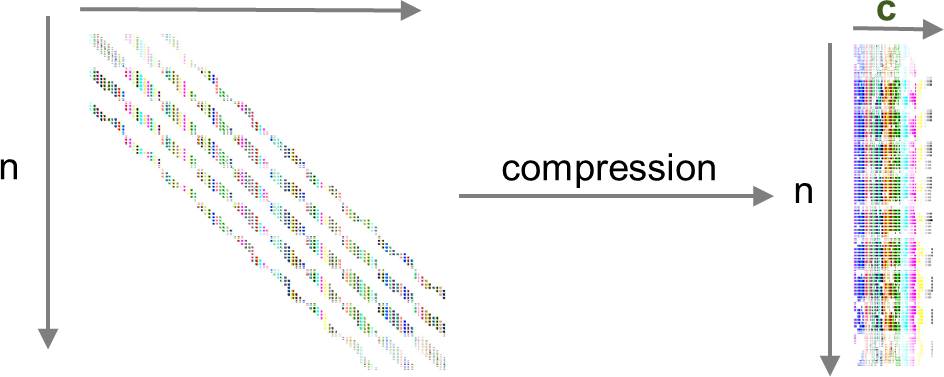
\includegraphics[width=0.45\textwidth]{figures/compression.png}
    \caption{Jacobian coloring}
    \label{fig:coloring}
\end{figure}

To avoid a complexity of $\bigo{n} \cdot cost(F)$ by letting the tangent mode
run over all Cartesian basis vectors of $\mathbb{R}^n$, we apply the technique of Jacobian
coloring to compress the sparse Jacobian \lstinline{J}. Running the tangent mode, it
allows to compute columns of the Jacobian concurrently, by combining
independent columns in one Jacobian-vector evaluation (see
\reffig{fig:coloring}). For sparsity detection we rely on the greedy
algorithm implemented by \lstinline{SparseDiffTools.jl} \cite{sparsedifftools}.

Given the sparsity pattern, the forward model is applied through the package
\lstinline{ForwardDiff.jl} \cite{RevelsLubinPapamarkou2016}. Given the number of Jacobian
colors $c$ we can build our dual type \lstinline{t1s} with \lstinline{c} directions:

\begin{lstlisting}[language = Julia]
t1s{N} = 
ForwardDiff.Dual{Nothing,Float64, N} where N}
\end{lstlisting}

Note that a second-order type \lstinline{t2s} can be created naturally by applying the same logic to \lstinline{t1s}:

\begin{lstlisting}[language = Julia]
t2s{M,N} =  
ForwardDiff.Dual{Nothing,t1s{N}, M} where M, N}
\end{lstlisting}

Finally, this dual type can be ported to both vector types \lstinline{Vector} and \lstinline{CuVector}:

\begin{lstlisting}[language = Julia]
VT = Vector{Float64}
VT = Vector{t1s{N}}}
VT = CuVector{t1s{N}}}
\end{lstlisting}

Setting \lstinline{VT} to either of the three types allows us to instantiate code that has been written using the {\it broadcast operator} \lstinline{.}

\begin{lstlisting}[language = Julia]
x .= a .* b
\end{lstlisting}

or accessed in kernels written with `KernelAbstractions.jl`, like for example the power flow equations (here in polar form):

\begin{lstlisting}[language = Julia]
@kernel function residual_kernel!(F, v_m, v_a,
                    re_nzval, re_colptr, re_rowval,
                    im_nzval, im_colptr, im_rowval,
                    pinj, qinj, pv, pq, nbus)

    npv = size(pv, 1)
    npq = size(pq, 1)

    i = @index(Global, Linear)
    # REAL PV: 1:npv
    # REAL PQ: (npv+1:npv+npq)
    # IMAG PQ: (npv+npq+1:npv+2npq)
    fr = (i <= npv) ? pv[i] : pq[i - npv]
    F[i] -= pinj[fr]
    if i > npv
        F[i + npq] -= qinj[fr]
    end
    for c in re_colptr[fr]:re_colptr[fr+1]-1
        to = re_rowval[c]
        aij = v_a[fr] - v_a[to]
        coef_cos = v_m[fr]*v_m[to]*re_nzval[c]
        coef_sin = v_m[fr]*v_m[to]*im_nzval[c]
        cos_val = cos(aij)
        sin_val = sin(aij)
        F[i] += coef_cos * cos_val 
              + coef_sin * sin_val
        if i > npv
            F[npq + i] += coef_cos * sin_val 
                        - coef_sin * cos_val
        end
    end
end
\end{lstlisting}

These two abstractions are a powerful tool that allow us to implement the
forward mode in vectorized form where the number of directions or tangent
components of a tangent variable are the number of Jacobian colors. We
illustrate this in \reffig{fig:simd} with a point-wise vector product \lstinline{x .* y}

\begin{figure}
    \centering
    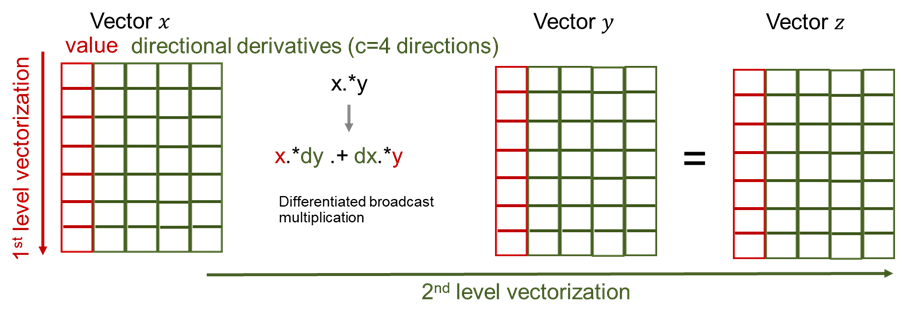
\includegraphics[width=0.45\textwidth]{figures/simd.png}
    \caption{SIMD AD for point-wise vector product}
    \label{fig:simd}
\end{figure}

This natural way of computing the compressed Jacobian yields a very high
performing code that is portable to any vector architecture, given that a
similar package like \lstinline{CUDA.jl} exists. We note that similar packages for the
Intel Compute Engine (\lstinline{oneAPI.jl}) and AMD ROCm (\lstinline{AMDGPU.jl}) are in development.
We expect our package to be portable to AMD and Intel GPUs in the future.

\subsection{Linear Solver}

As mentioned before, a linear solver is required to compute the Newton step in

\begin{lstlisting}[language = Julia]
dx .= jacobian(x)\F(x)
\end{lstlisting}

Our package supports the following linear solvers:

\begin{itemize}
    \item CUSOLVER with `csrlsvqr` (GPU),
    \item `Krylov.jl` with `dqgmres` (CPU/GPU),
    \item `IterativeSolvers` with `bicgstab` (CPU) [@sleijpen1993bicgstab],
    \item UMFPACK through the default Julia `\` operator (CPU),
    \item and a custom BiCGSTAB implementation [@bicgstabVorst] (CPU/GPU).
\end{itemize}

The last custom implementation was necessary as BiCGSTAB showed much better
performance than GMRES and at the time of this writing both \lstinline{Krylov.jl} and
\lstinline{IterativeSolvers.jl} did not provide an implementation that supported
\lstinline{CUDA.jl}.

Using the iterative solver out of the box leads to divergence and bad performance due to
ill-conditioning of the Jacobian. This is a known phenomenon in power
systems. That is why this package comes with a block Jacobi preconditioner
that is tailored towards GPUs and is proven to work well with power flow
problems.

The Jacobian is partitioned into a dense block diagonal structure, where each block is inverted to build our preconditioner \lstinline{P}. For the partition we use \lstinline{Metis.jl}.

\begin{figure}
    \centering
    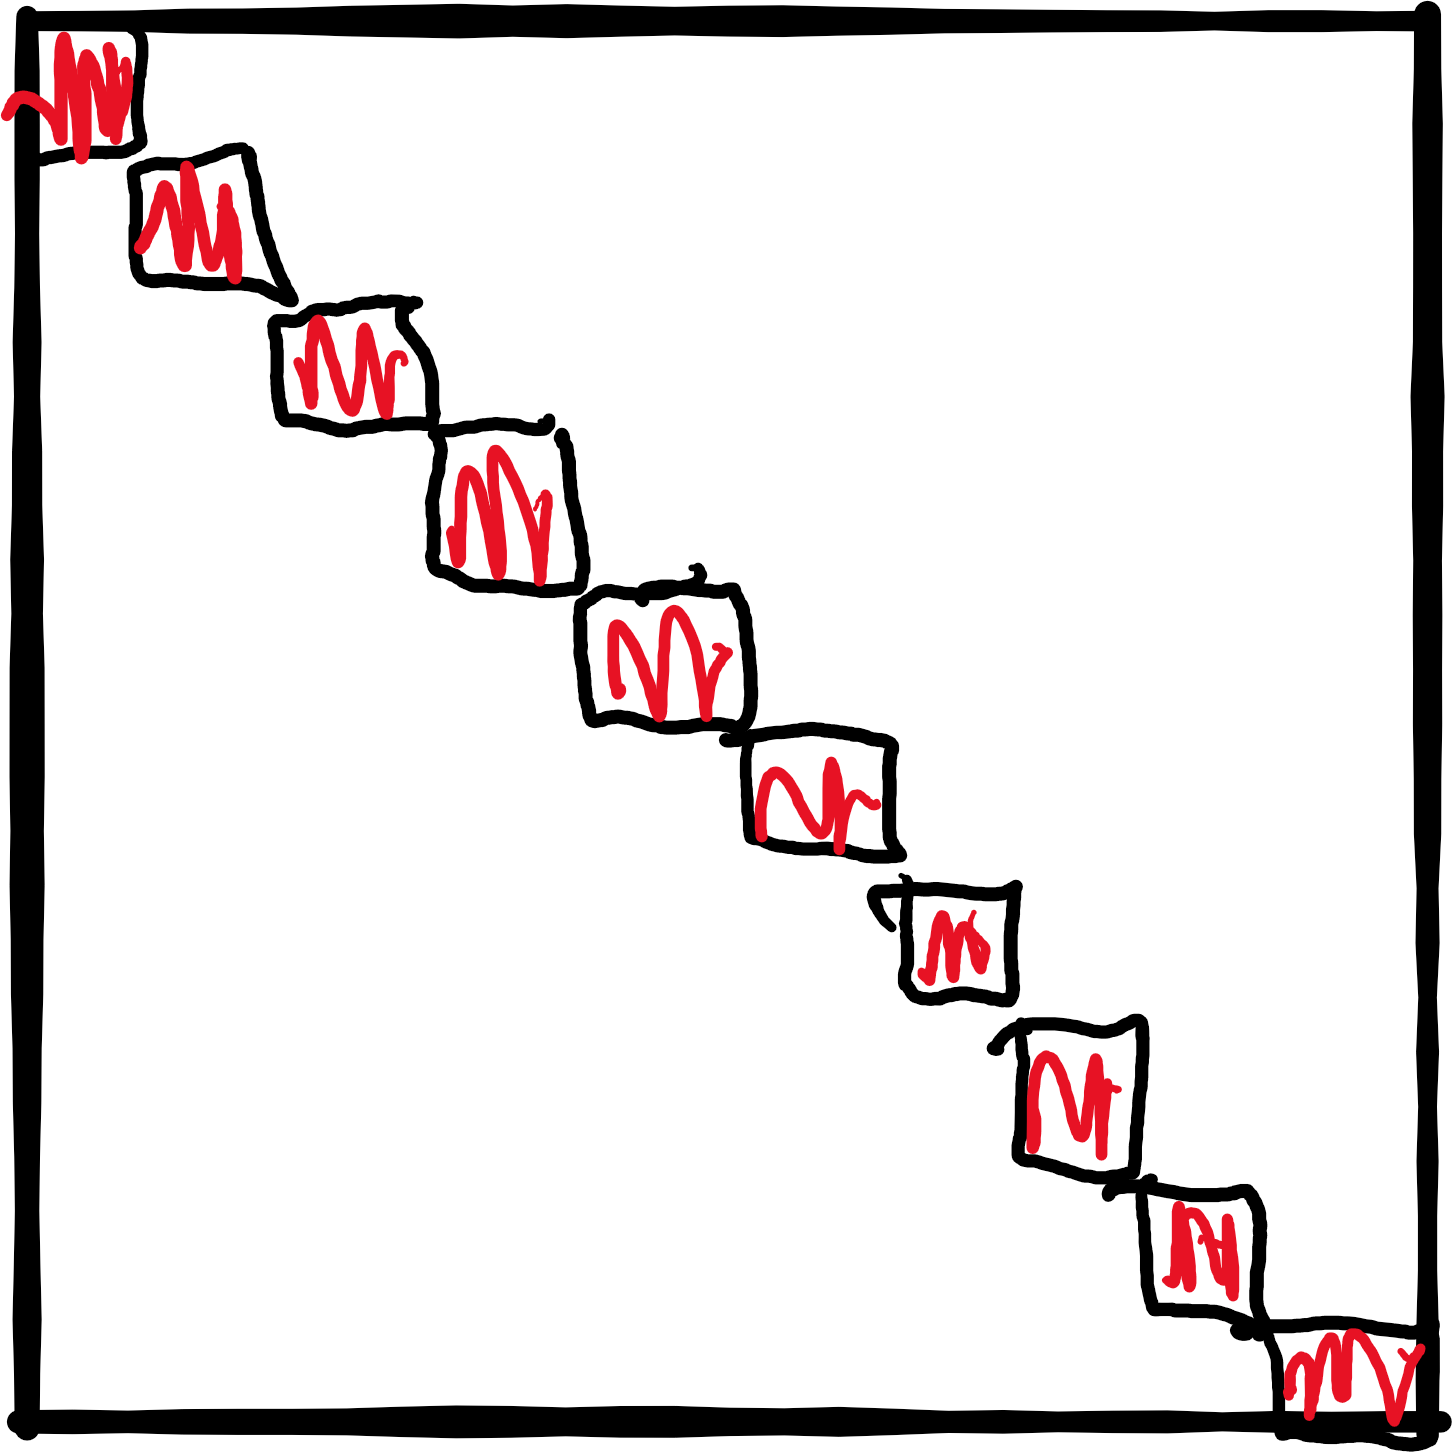
\includegraphics[width=0.25\textwidth]{figures/gpublocks.png}
    \caption{Dense block Jacobi preconditioner}
    \label{fig:preconditioner}
\end{figure}

Compared to incomplete Cholesky and incomplete LU this preconditioner is easily portable to the GPU if the number of blocks is high enough. \lstinline{ExaPF.jl} uses the batch BLAS calls from \lstinline{CUBLAS} to invert the single blocks.

\begin{lstlisting}[language = Julia]
CUDA.@sync pivot, info = 
CUDA.CUBLAS.getrf_batched!(blocks, true)
CUDA.@sync pivot, info, p.cuJs = CUDA.CUBLAS.getri_batched(blocks, pivot)
\end{lstlisting}

Assuming that other vendors will provide such batched BLAS APIs, this code is portable to other GPU architectures.

\section{Performance Example}

To get an impression of the use case for this solver we consider a 30,000 bus system case from the ARPA-E GO competition.
We show how the convergence of the BiCGSTAB algorithm is impacted by the number of blocks in the Jacobi preconditioner.
By choosing appropriately the number of blocks, we observe that the iterative solver
takes 0.55s to solve the linear system on the GPU. As a comparison,
LAPACK takes 0.22s to solve the system on the CPU, and CUSOLVER (with \lstinline{csrlsvqr})
takes 2.70s.

\begin{figure}
    \centering
    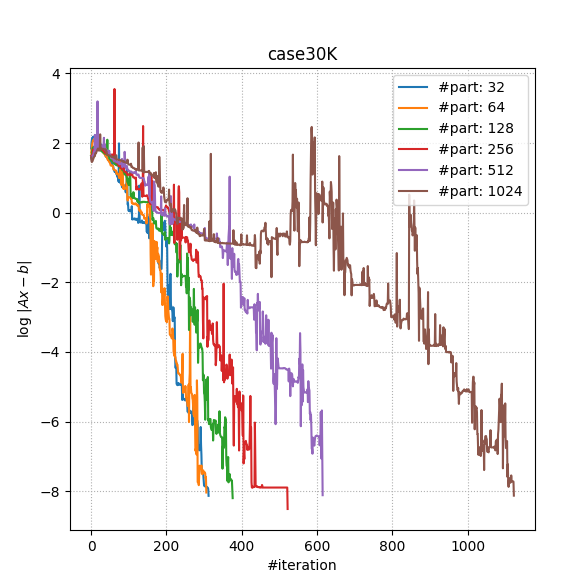
\includegraphics[width=0.45\textwidth]{figures/usecase.png}
    \caption{Use Case}
    \label{fig:usecase}
\end{figure}

\begin{table}[t]
    \begin{tabular}{ccccc}
    Blocks & Block Size & Time(s) &  Time/It.(s) & \#Iterations \\
    \hline
    32 &   1857 &       2.85e+00 &  9.07e-03 &  314 \\
    64 &   928  &       1.41e+00 &  4.57e-03 &  308 \\
    128 &   464  &       9.15e-01 &  2.42e-03 &  378 \\
    256 &   232  &       9.09e-01 &  1.74e-03 &  524 \\
    512 &   116  &       5.49e-01 &  8.90e-04 &  617 \\
    1024 &   58   &       7.50e-01 &  6.67e-04 & 1125 \\
    \end{tabular}
\end{table}


This shows the number of BiCGSTAB iterations and the time needed to achieve convergence for this power system.

\section{Acknowledgments}

This research was supported by the Exascale Computing Project (17-SC-20-SC), a joint project of the U.S. Department of Energy’s Office of Science and National Nuclear Security Administration, responsible for delivering a capable exascale ecosystem, including software, applications, and hardware technology, to support the nation’s exascale computing imperative.

\bibliographystyle{juliacon}
\bibliography{ref}

% \section{Additional features}
% \label{sec:additional_faci}
% In addition to all the standard \LaTeX{} design elements, the \verb juliacon  class file includes the following features:
% In general, once you have used the additional \verb juliacon.cls facilities
% in your document, do not process it with a standard \LaTeX{} class
% file.

% \subsection{Titles, Author's Name, and Affiliation}
% \label{subsub:title_auth}
% The title of the article, author's name, and affiliation are used at the
% beginning of the article (for the main title). These can be produced
% using the following code:

% \begin{verbatim}
% \title{ This is an example of article title} }
% \author{
%    \large 1st Author \\[-3pt]
%    \normalsize 1st author's affiliation  \\[-3pt]
%     \normalsize 1st line of address \\[-3pt]
%     \normalsize 2nd line of address \\[-3pt]
%     \normalsize	1st author's email address \\[-3pt]
%   \and
%    \large 2nd Author \\[-3pt]
%    \normalsize 2nd author's affiliation  \\[-3pt]
%     \normalsize 1st line of address \\[-3pt]
%     \normalsize 2nd line of address \\[-3pt]
%     \normalsize	2nd author's email address \\[-3pt]
% \and
%    \large 3rd Author \\[-3pt]
%    \normalsize 3rd author's affiliation  \\[-3pt]
%     \normalsize 1st line of address \\[-3pt]
%     \normalsize 2nd line of address \\[-3pt]
%     \normalsize	3rd author's email address \\[-3pt]
% }
% \maketitle
% \end{verbatim}
% \label{subsub:references}
% References are most easily (and correctly) generated using the
% BIBTEX, which is easily invoked via
% When submitting the document source (.tex) file to external
% parties, the ref.bib file should be sent with it.
% \cite{bezanson2017julia}

% % **************GENERATED FILE, DO NOT EDIT**************

\bibliographystyle{juliacon}
\bibliography{ref.bib}


\end{document}

% Inspired by the International Journal of Computer Applications template
